%%%%%%%%%%%%%%%%%%%%%%%%%%%%%%%%%%%%%%%%%%%%%%%%%%%%%%%%%%%%%%%%%%%%
%%%%% HEADER %%%%%
%%%%%%%%%%%%%%%%%%%%%%%%%%%%%%%%%%%%%%%%%%%%%%%%%%%%%%%%%%%%%%%%%%%%

\documentclass[a4paper]{article}


%%%%% Packages %%%%%

	%%%%% Language %%%%% 
\usepackage[frenchb]{babel}
\usepackage[utf8]{inputenc}
\usepackage[T1]{fontenc}
	%%%%% Graphic %%%%%
\usepackage{graphicx}
	%%%%% Mise en page %%%%%
\usepackage{fancyhdr}
	%%%%% Tableaux %%%%%
\usepackage{colortbl} 

%%%%% Macros %%%%
\newcommand{\HRule}{\rule{\linewidth}{0.5mm}}

\pagestyle{fancy}
\lhead{EMF Project \\ Projet de Vérification et tests}
\rhead{Coraline \textsc{Marie} \\ Vincent \textsc{Raveneau}}

%%%%% Doc's informations %%%%%


%%%%%%%%%%%%%%%%%%%%%%%%%%%%%%%%%%%%%%%%%%%%%%%%%%%%%%%%%%%%%%%%%%%%
%%%%% DOCUMENT %%%%%
%%%%%%%%%%%%%%%%%%%%%%%%%%%%%%%%%%%%%%%%%%%%%%%%%%%%%%%%%%%%%%%%%%%%

\begin{document}

	%%%%% Page de garde %%%%
	\begin{titlepage}
		\begin{center}

			
\includegraphics[width=0.45\textwidth]{UN-sciences.png}~\\[2cm]

			\LARGE{Master 1 \sc{Alma}}\\[1.5cm]

			\Large{Projet de Vérification et tests}\\[0.5cm]

			% Titre
			\HRule \\[0.4cm]
			{ \huge \bfseries EMF Project \\[0.4cm] }
			\HRule \\[1.5cm]

			% Auteur et Encadrant
			\normalsize		
			\emph{\'Etudiants :}\\
			Coraline \textsc{Marie} et Vincent \textsc{Raveneau}\\
			\vspace{0.5cm}
			\emph{Intervenant :} \\
			Gerson \textsc{Sunyé}
		
			\vfill

			% Bottom of the page
			{\large 13 décembre 2013}

		\end{center}
	\end{titlepage}


	%%%%% Sommaire %%%%%
	\renewcommand{\contentsname}{Sommaire}
	\tableofcontents
	\newpage


	%%%%% Introduction %%%%%
	\begin{center}
		\section{Introduction}
	\end{center}

	\vspace{0.5cm}

	La création d'un logiciel, quel qu'il soit, n'est jamais sûr. Le code source peut contenir des fautes, des bugs ou des défauts, sans même que le programmeur ne les remarque. Fort heureusement, il existe aujourd'hui des méthodes efficaces pour contrer ces failles, et renforcer la fiabilité du code source, comme par exemple les tests unitaires.

	\vspace{0.5cm}

	Le module \textit{Vérification et Tests} que nous avons étudié en Master \textsc{Alma} à l’Université de Nantes, nous a apporté un ensemble de techniques utilisables sur la majorité des langages informatique. Pour parfaire cet apprentissage, nous avons travaillé sur la restructuration et l'amélioration de l'EMF (Eclipse Modeling Framework), un logiciel libre développé pour et par Eclipse.

	\vspace{0.5cm}

	Ce rapport présente donc une application directe de ce que nous a appris le module Vérification et tests, au travers de deux grandes étapes de travail. Pour la première, nous avons tout d'abord restructuré une partie du code source de l'EMF en un projet Maven. Puis nous avons évalué les tests déjà présent dans ce code. Pour la seconde étape nous avons amélioré autant que possible la qualité de la classe URI, afin d'augmenter sa fiabilité.

	\newpage


	%%%%% Partie 1 %%%%%
	\begin{center}
		\section{Restructuration et évaluation}
	\end{center}

	\vspace{0.5cm}

		%%%%% Partie 1.1 %%%%%
		\subsection{Réorganisation avec Maven}

		\vspace{0.5cm}

		L'un des objectifs pédagogiques du projet de vérification et tests, était de nous apprendre à utiliser un nouvel outil : Maven. 

		\subsubsection{Qu'est ce que Maven ?}

		\vspace{0.5cm}

		Maven (ou Apache Maven) est un logiciel libre, qui permet la gestion et la production automatique de projets liés au langage de programmation Java. Il s'agit d'un outil, qui aide à la conception de logiciels à partir du code source, en optimisant les tâches et en garantissant le bon ordre de fabrication.

		\vspace{0.5cm}

		\subsubsection{Convertion du code original}

		\vspace{0.5cm}

		Le code source original du projet EMF est disponible sur gitHub. Il est donc téléchargeable en archive, et modifiable par n'importe qui. Cependant, l'archive que nous avons récupérée fournit un code source conditionné pour l'environnement de développement Eclipse, et cet IDE nous a été fortement déconseillé.

		\vspace{0.5cm}

		Ainsi, pour répondre à la demande du cahier des charges de ne pas utiliser Eclipse, nous avons choisi un nouvel IDE compatible avec Maven pour travailler. Ce choix s'est porté sur l'IDE NetBeans, qui permet de supporter plusieurs langages, et dont la dernière version inclut Maven. Cependant, le code source original devait être au préalable adapté, avant de pouvoir le travailler.

		\vspace{0.5cm}

		Afin d'optimiser notre travail, nous n'avons pas converti la totalité de l'archive téléchargée, mais juste la partie du code intéressante pour le projet. Malgré la facilité de conversion de l'architecture, cette tâche fût longue et relativement fastidieuse. Certaines erreurs de package et de plugin sont apparues, ce qui nous a pris du temps à résoudre. 

		\vspace{0.5cm}

		Voici l'arborescance obtenue après la conversion du code source original en projet Netbean/Maven : 

		\begin{center}
			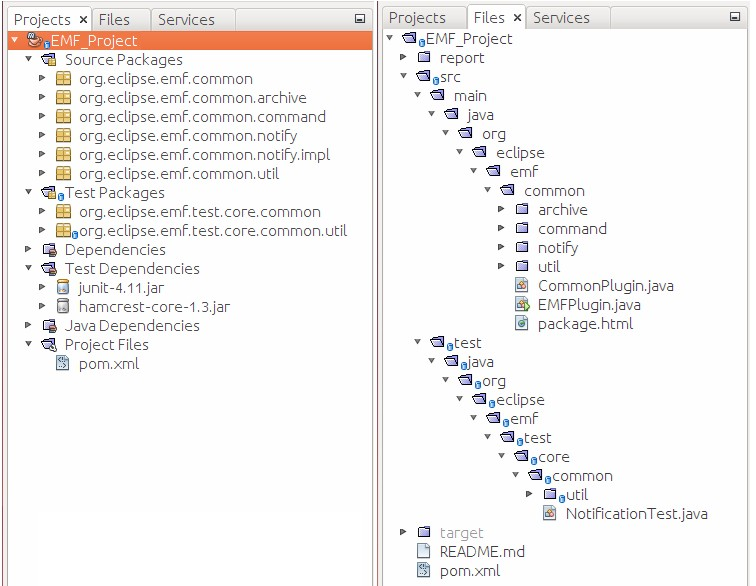
\includegraphics[width=1.0\textwidth]{Arborescence.jpg}~\\
		\end{center}

		\vspace{0.5cm}

		\subsubsection{Bugs et résolution}

		\vspace{0.5cm}

		Pour gérer les bibliothèques et les dépendances d'un projet, Maven utilise un fichier \texttt{pom.xml}, qui décrit l'ensemble des besoins de l'application. Lors de la conversion du code source initial vers notre projet Maven, plusieurs erreurs liées à ce fichier sont apparues, car il manquait des dépendances :
		\begin{itemize}
			\item JUnit : framework de test unitaire.
			\item Core Runtime : framework (de Eclipse RCP).
			\item EMF ecore et EMF ecore xmi.
		\end{itemize}

		\vspace{0.5cm}



		%%%%% Partie 1.2 %%%%%
		\subsection{Evaluation des tests}

		\vspace{0.5cm}

		Après avoir lancé les tests, déjà présents dans l'archive initiale, plusieurs problèmes sont apparus. Tout d'abord, il y a eu très peu de couverture du code par les tests (d'après l'IDE Netbeans, moins de 40 \% du code est couvert). Ce problème est principalement dû au fait qu'il y ait deux classes de tests, qui possèdent chacune des dépendances que l'on ne peut pas satisfaire. De plus, le logiciel qui permet de tester efficacement les mutations, ne fonctionne pas correctement, et n'exécute pas les bons tests.

	\newpage

	%%%%% Partie 2 %%%%%
	\begin{center}
		\section{Amélioration de URI}
	\end{center}

	\vspace{0.5cm}

		%%%%% Partie 2.1 %%%%%
		\subsection{La classe URI}

		\vspace{0.5cm}

			\subsubsection{Défauts de conception}

			Bla bla bla bla bla

			\vspace{0.5cm}

			\subsubsection{Améliorations possibles}

			Bla bla bla bla bla

			\vspace{0.5cm}


		%%%%% Partie 2.2 %%%%%
		\subsection{Modifications}

		\vspace{0.5cm}

		Bla bla bla bla bla


\end{document}
